\chapter{EBOA interface}

\acrshort{eboa} offers interfaces for 3 general operations with data: insert, update and query.

This data can be provided in three formats: XML, JSON and Python dictionary. This data is verified against a schema so that the data is checked before processing it. The XML schema can be seen in appendix \ref{ap:xml_schema} and the JSON and python schema can be seen in appendix \ref{ap:json_schema}

\section{Insert interface}

\acrshort{eboa} offers an interface for inserting data filling the tables shown in the data model included in figure \ref{fg:eboadb}.

\section{Python insert interface}

In this section, the Python interface for inserting data is explained.

The entry point for inserting data using the Python interface is the following method:

\begin{lstlisting}[style=python]
    def treat_data(self, data = None, source = None, validate = True):
        """
        Method to treat the data stored in self.data
        :param data: structure of data to treat
        :type data: dict 
        :param source: name of the source of the data
        :type source: str
        :param validate: flag to indicate if the schema check has to be performed
        :type validate: bool
        """  
\end{lstlisting}

So, for example for inserting data using the python interface the following code could be executed:

\begin{lstlisting}[style=python]
from eboa.engine.engine import Engine

engine = Engine()

data = {"operations": [{
    "mode": "insert",
    "dim_signature": {"name": "dim_signature",
                      "exec": "exec",
                      "version": "1.0"},
    "source": {"name": "source.xml",
               "generation_time": "2018-07-05T02:07:03",
               "validity_start": "2018-06-05T02:07:03",
               "validity_stop": "2018-06-05T08:07:36"},
    "events": [{
        "explicit_reference": "EXPLICIT_REFERENCE_EVENT",
        "gauge": {"name": "GAUGE_NAME",
                  "system": "GAUGE_SYSTEM",
                  "insertion_type": "SIMPLE_UPDATE"},
        "start": "2018-06-05T02:07:03",
        "stop": "2018-06-05T08:07:36"
    }],
    "annotations": [{
        "explicit_reference": "EXPLICIT_REFERENCE_ANNOTATION",
        "annotation_cnf": {"name": "NAME",
                           "system": "SYSTEM"}
    }]
}]}

returned_value = engine.treat_data(data)
\end{lstlisting}

And the result would be the insertion of:
\begin{itemize}
\item One entry into the table dim\_signature\_tb
\item One entry into the table dim\_processing\_tb
\item One entry into the table dim\_processing\_status\_tb
\item One entry into the table event\_tb
\item One entry into the table explicit\_reference\_tb
\item One entry into the table gauge\_cnf\_tb
\item One entry into the table annotation\_tb
\item One entry into the table annotation\_cnf\_tb
\end{itemize}

\section{Events ingestion}

Events can be inserted following 3 different methods associated to their gauges:

\begin{itemize}
\item SIMPLE\_UPDATE: all events are inserted
\item ERASE\_and\_REPLACE: all the events are inserted but flagged as not visible. Then the \acrshort{eboa} checks the events falling in the validity period of the source of the events just inserted into the DDBB, with the same gauge and keeps the events with greatest generation time and removes the rest. In case an event does not fully fall in the validity period and has to be removed, the event is split so that the part not falling into the validity period remains.
\item EVENT\_KEYS: the events are inserted but flagged as not visible. Then the \acrshort{eboa} checks the events with the same event key and same DIM signature and keeps the ones with the greatest generation time.
\end{itemize}

\subsection {ERASE\_and\_REPLACE method}

In this section, an example of the behaviour is shown in figure \ref{fg:erase_and_replace_algorithm} and described in table \ref{tb:erase_and_replace_algorithm}. The bubbles in the figure represent events and the line beneath them the validity period of their corresponding source of information. All the events have the same gauge configuration.
The events are firstly inserted flagged as not visible. Then, the method, after applying the algorithm described bellow, is in charge of deleting the events or making them visible.
The steps of the algorithm are as follows:

\begin{enumerate}

\item The algorithm iterates over the gauges inserted with mode ERASE\_and\_REPLACE
\item \label{for_each_gauge} For each gauge inserted with mode ERASE\_and\_REPLACE, the algorithm gets all the validity periods of the sources associated to the events falling into the validity period of the source associated to the events just inserted with this gauge
\item The algorithm sets a timeline with the start and stop values of the validities
\item The algorithm iterates over every timestamp of the timeline
\item If the timestamp is the last one of the timeline, the algorithm copies every event inside the list "List of split" into the list "List to be created" with the start value equal to the timestamp and inserts the event into the list "List to be removed". Once this step is finised, it goes to step \ref{for_each_gauge}
\item The algorithm gets the greatest generation time from the sources which events fall into the period between the actual timestamp and the following one
\item The algorithm iterates over the events corresponding to the greatest generation time
\item If the event is inside the list "List of split": if the stop of the event is lower or equal to the stop of the current period, then the event is inserted into the list "List to be created" with the start modified to be the start of the current period. The event is removed from the list "List of split".
\item If the event is inside the list "List of split": if the stop of the event is greater than the stop of the current period, then the event is inserted into the list "List to be created not ending on the current period" with a start value equal to the start of the current period. The event is removed from the list "List of split".
\item If the event is not inside the list "List of split", the event is made visible
\item The algorithm deletes all the events fully contained in the period which source has a generation time lower than the greatest
\item The algorithm iterates over all the events not fully contained in the period which source has a generation time lower than the greatest
\item If the event is not in the list "List of split", the algorithm goes to step \ref{event_starts_before}. Otherwise it goes to step \ref{event_starts_after}
\item \label{event_starts_before} If the start of the event is lower than the start of the period, the algorithm copies the event into the list "List to be created". If the event is on the list "List to be created not ending on the current period", the start of the event is equal to the start of the period when the event was inserted into this list (the copy inside the list "List to be created not ending on the period" is removed). Otherwise the start is the start of the event
\item If the stop of the event is greater than the stop of the period, the event is inserted into the list "List of split" and marked as not visible. Otherwise the event is inserted into the list "List to be removed"
\item \label{event_starts_after} If the stop of the event is lower or equal to the stop of the current period, the event is inserted into the list "List to be removed" and removed from the list "List of split"
\item The algorithm goes to step \ref{for_each_gauge}
\end{enumerate}

\begin{figure}[H]
  \begin{center}
	\centering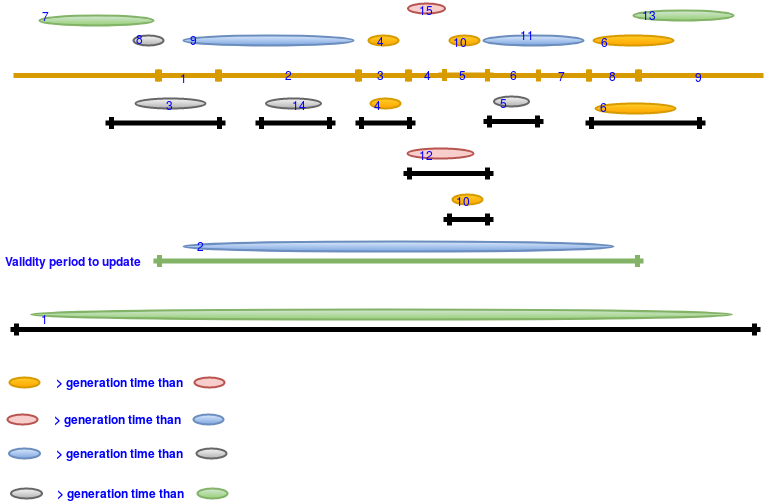
\includegraphics[width=150mm]{../fig/erase_and_replace_algorithm.png}
	\caption{Example of the effect of the erase and replace operation}
	\label{fg:erase_and_replace_algorithm}
  \end{center}
\end{figure}

\begin{table}[H]
\begin{tabular}{|M{0.07\linewidth}|M{0.15\linewidth}|M{0.15\linewidth}|M{0.15\linewidth}|M{0.15\linewidth}|M{0.15\linewidth}|M{0.15\linewidth}|}
\hline
Period & List to be created  & List to be created not ending on the current period & List to be removed & List of split & Marked as visible \\ \hline
1      & 7, 8                & -                                                   & 3                  & 1             & 2                 \\ \hline
2      & 7, 8                & -                                                   & 3, 14              & 1             & 2                 \\ \hline
3      & 7, 8, 9             & -                                                   & 3, 14              & 1, 2          & 4                 \\ \hline
4      & 7, 8, 9             & -                                                   & 3, 14              & 1, 2          & 4, 12             \\ \hline
5      & 7, 8, 9, 15         & -                                                   & 3, 12, 14          & 1, 2          & 4, 10             \\ \hline
6      & 7, 8, 9, 15         & 11                                                  & 3, 5, 12, 14       & 1             & 2, 4, 10          \\ \hline
7      & 7, 8, 9, 15         & 11                                                  & 3, 5, 12, 14       & 1             & 2, 4, 10          \\ \hline
8      & 7, 8, 9, 11, 15     & -                                                   & 2, 3, 5, 12, 14    & 1             & 4, 6, 10          \\ \hline
9      & 7, 8, 9, 11, 13, 15 & -                                                   & 2, 3, 5, 12, 14    & 1             & 4, 6, 10          \\ \hline
\end{tabular}
\caption{Table showing the steps done by the erase and replace algorithm}
\label{tb:erase_and_replace_algorithm}
\end{table}


\subsection {EVENT\_KEYS method}

The algorithm used to insert events using the method EVENT\_KEYS is a lot less complex than the algorithm used to insert events using the method ERASE\_and\_REPLACE.
The events and the associated keys are firstly inserted flagged as not visible. The method after applying the algorithm described bellow is in charge of deleting the events or making them visible, as well as making the event keys visible.
This method considers the generation time of the source associated to the events just inserted and its DIM signature assciated joint with every event key.
The steps are as follows:

\begin{enumerate}

\item The algorithm iterates over the pairs (event key, DIM signature UUID)
\item \label{for_each_pair} For each pair associated to events inserted with mode EVENT\_KEYS, the algorithm gets the first event associated to the event key and the DIM signature UUID which source has the greatest generation time
\item The algorithm deletes the rest of events associated to the event key and the DIM signature UUID and which source is different than the source of the previous event
\item The algorithm makes visible the events and the event keys associated to the source of the event with the greatest generation time
\item The algorithm goes to step \ref{for_each_pair}
\end{enumerate}

\section{Annotations ingestion}

Annotations are inserted associated to their explicit references and their annotation configuration.
The method followed for inserting annotations is similar to the method used for inserting events using the method EVENT\_KEYS.
The annotations are firstly inserted flagged as not visible. The method after applying the algorithm described bellow is in charge of deleting the annotations or making them visible.
The steps are as follows:

\begin{enumerate}

\item The algorithm iterates over the tuples (annotation configuration name, annotation configuration system, explicit reference)
\item \label{for_each_tuple} For each tuple associated to an inserted annotation inserted, the algorithm gets the first annotation associated to the annotation configuration and the explicit reference which source has the greatest generation time
\item The algorithm deletes the rest of annotations associated to the annotation configuration and the explicit reference and which source is different than the source of the previous annotation
\item The algorithm makes visible the annotations associated to the source of the annotation with the greatest generation time
\item The algorithm goes to step \ref{for_each_tuple}
\end{enumerate}


